% 第6章 評価
\newpage
\renewcommand{\baselinestretch}{1.5}
\section{評価}
\renewcommand{\baselinestretch}{1}

本手法を評価する為に3つの実験を20代の大学生・大学院生10人に対して実施した。被験者はいずれも日常的にインターネットを使用するネットユーザーであった。

\subsection{評価方法}
\subsubsection{重要領域の抜き出し精度に関する評価}
\par 1つ目の評価方法では本手法の重要領域の抜き出しの精度を測る為に、10個のウェブページのスクリーンショットをi-Pad上に表示して10秒以内に目立つ・目に入ったと感じた領域3箇所に1$\sim$3の数字を順番にApple pencilを使用してマークしてもらう実験を実施した。日常的に利用するウェブページを実験対象とすると経験則に基づく偏見が結果に反映されてしまう恐れがある為、日本のウェブページのデザインを業界カテゴリに分けて紹介しているJapan Web Design Gallery\cite{japanwebgallery}の業種カテゴリの中からランダムに選んだカテゴリの最初に表示されたウェブページを実験対象に使用した。ただし、アニメーションなどにより要素が常に動いているものや全画面が1枚の画像や動画のみで構成されているものは本システムでは評価できない為使用しなかった。実験に使用した10個のウェブサイトの一覧を表\ref{table:webpage-list}に、またそのスクリーンショットを図\ref{fig_evaluation-webpage}に示す。


\begin{table}[h]
    \caption{精度評価実験に使用したウェブページの一覧(全て2019年1月20日閲覧)}
    \label{table:webpage-list}
    \centering
    \begingroup
    \renewcommand{\arraystretch}{1.1} % 表の行間の変更
    \small
     \begin{tabular}{llll}
      \hline
      & ページ名 & カテゴリ & URL \\
      \hline \hline
      A & アクロス福岡 & ホール・劇場 & https://www.acros.or.jp/ \\
      B & カキモリ & クリエイティブ & http://kakimori.com/ \\
      C & 株式会社ヒビノ & 音楽・楽器 & https://www.hibino.co.jp/ \\
      D & 上越市立水族館 & 水族館 & http://umigatari.jp/joetsu/ \\
      E & PLEXLOGGER & カメラ & http://plextor.jp/plexlogger/ \\
      F & 川崎市民交流センター & ホール・劇場 & https://s-tette.jp/ \\
      G & 株式会社まちづくり長野 & まちづくり & http://machidukuri-nagano.jp/ \\
      H & 渋谷ストーム & 不動産 & https://shibuyastream.jp/ \\
      I & 司法書士青木事務所 & 会計・法律 & https://aoki-jimusho.net/ \\
      J & 東北芸術工科大学 & 大学・専門学校 & https://www.tuad.ac.jp/ \\
      \hline
    \end{tabular}
    \endgroup
\end{table}


\begin{figure}[H]
    \centering
    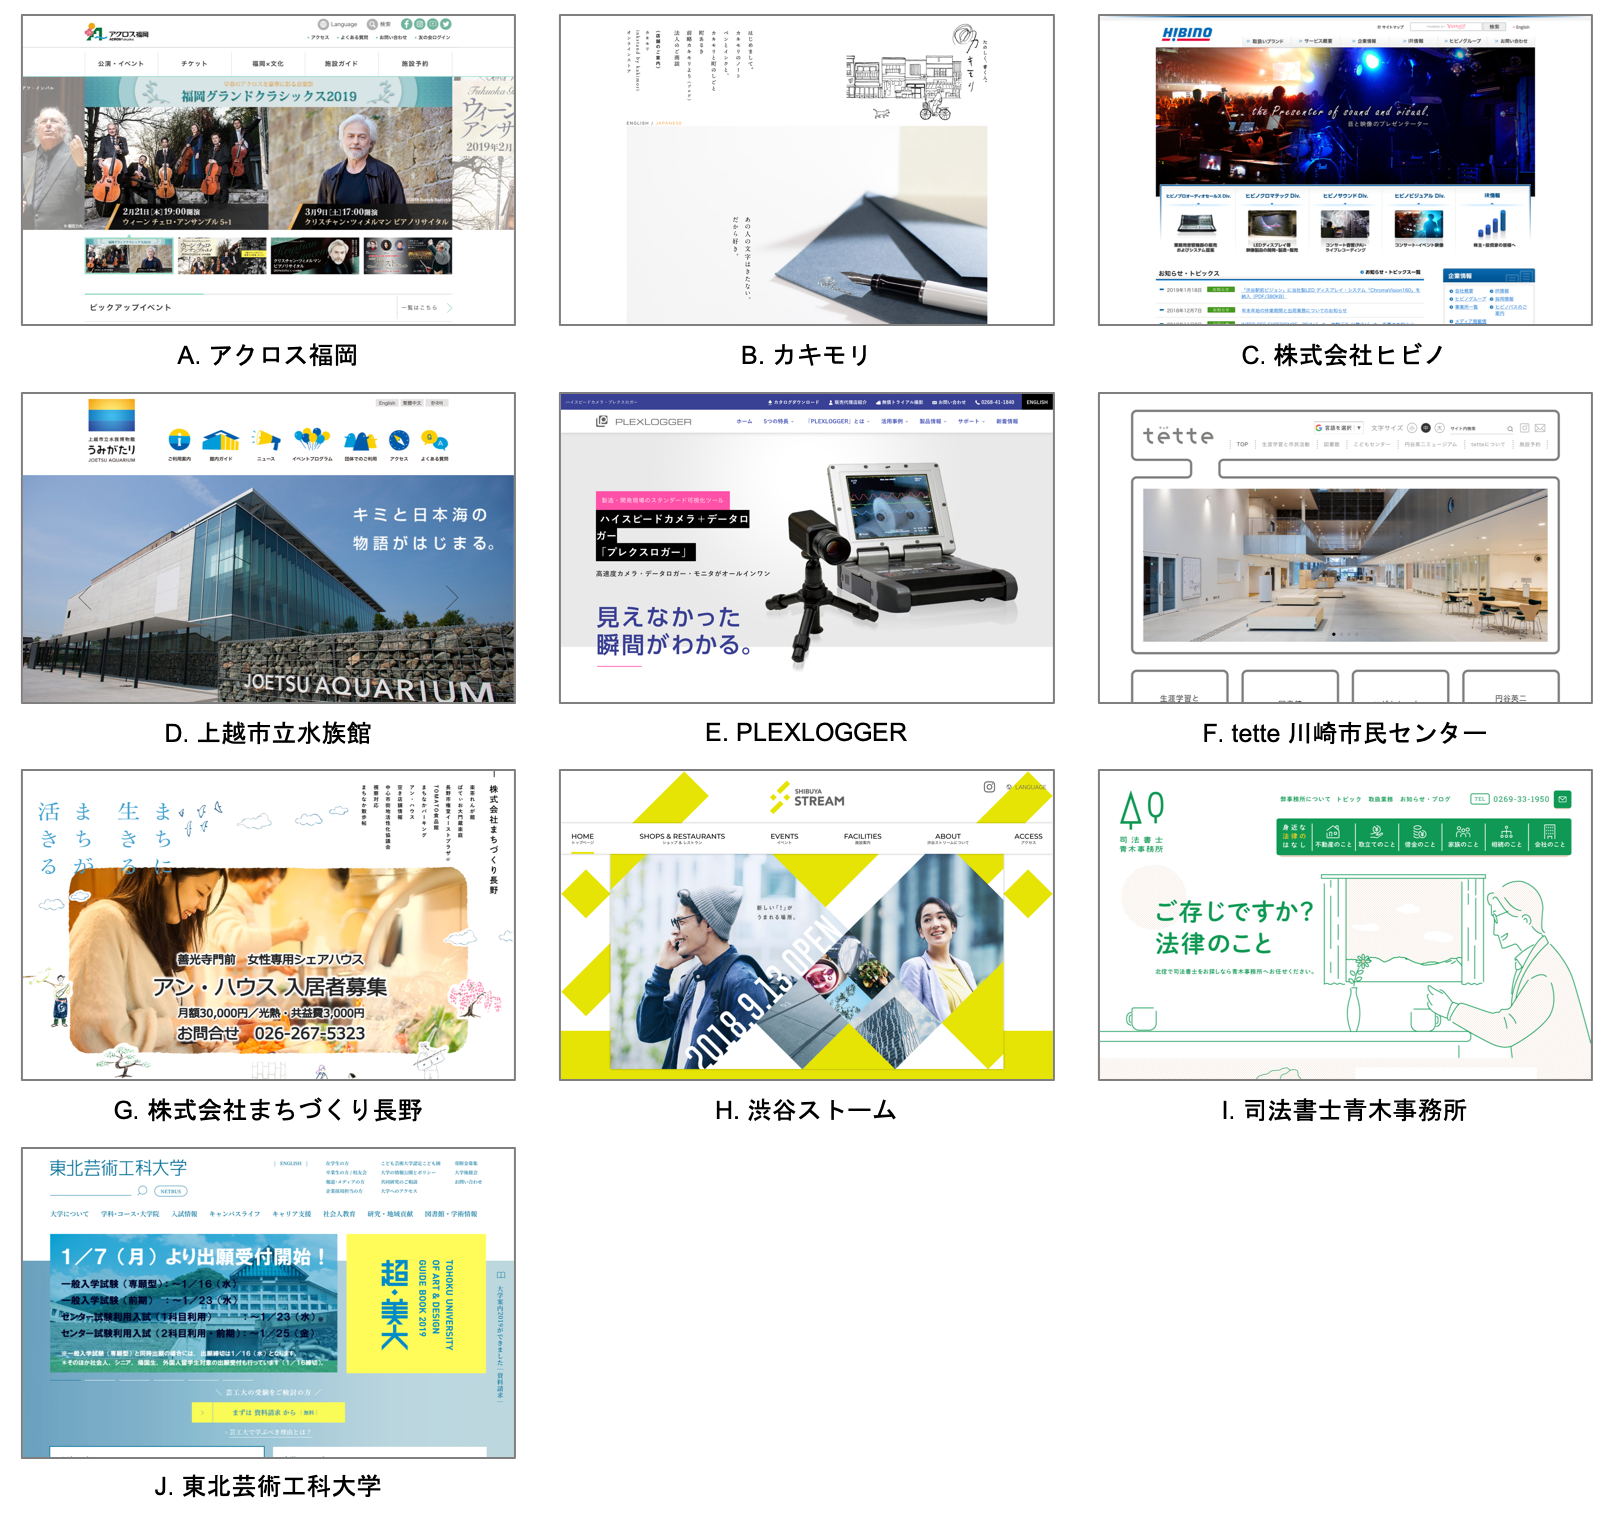
\includegraphics[width=12cm]{figures/webpage.png}
    \caption{使用したウェブページのスクリーンショット}
    \label{fig_evaluation-webpage}
\end{figure}

\subsubsection{重要領域の認識のしやすさに関する評価}
\par 2つ目の評価方法では既存の顕著性マップと提案手法の顕著領域マップでの重要領域の認識のしやすさについて評価した。評価では顕著性マップの概要について簡単に説明した後に図\ref{fig_experience02}に示すJapan Web Design Gallery\cite{japanwebgallery}に掲載されている2つのウェブページの既存の顕著性マップと提案手法の顕著領域マップの例を提示して、最後に\ref{table:question01}に示すアンケートを実施した。アンケートでは既存の顕著性マップと提案手法の顕著領域マップの重要領域の認識のしやすさの度合いと、どのような点で認識しやすく感じたり認識しにくいと感じるのかを記述式で質問した。実験に使用した2つのウェブページ情報を表\ref{table:webpage-list2}に示す。


\begin{table}[h]
    \caption{重要領域認識実験に使用したウェブページの一覧(全て2019年1月20日閲覧)}
    \label{table:webpage-list2}
    \centering
    \begingroup
    \renewcommand{\arraystretch}{1.2} % 表の行間の変更
    \small
     \begin{tabular}{llll}
      \hline
      & ページ名 & カテゴリ & URL \\
      \hline \hline
      K & 下関春帆楼 & カフェ・レストラン & https://www.shunpanro.com/ \\
      L & 白洋舎 & クリーニング & http://www.hakuyosha.co.jp/ \\
      \hline
    \end{tabular}
    \endgroup
\end{table}



\begin{figure}[H]
    \centering
    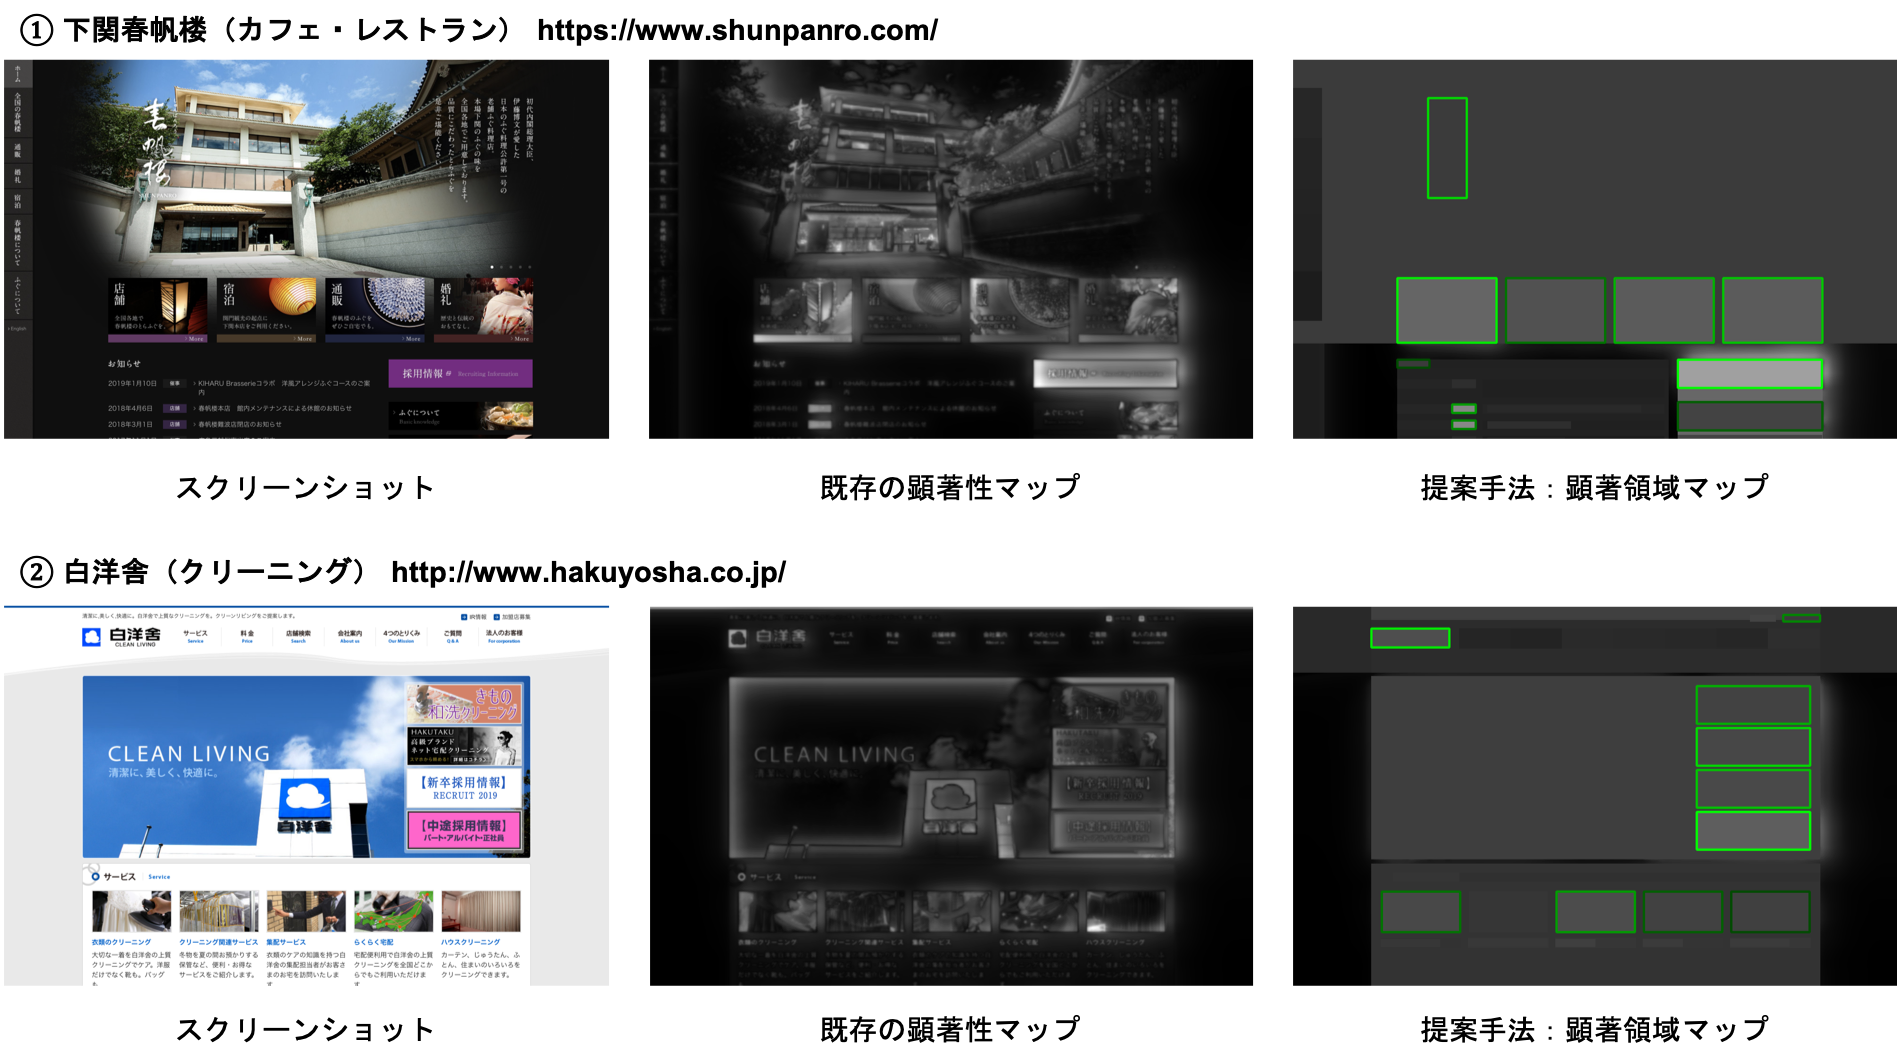
\includegraphics[width=12cm]{figures/experience02.png}
    \caption{既存の顕著性マップと提案手法(顕著領域マップ)の比較実験}
    \label{fig_experience02}
\end{figure}

\begin{table}[h]
    \caption{アンケートの質問内容1}
    \label{table:question01}
    \centering
    \begingroup
    \renewcommand{\arraystretch}{1} % 表の行間の変更
    \small
    \begin{tabular}{|l|l|l|l|}
        \hline
        \multicolumn{2}{|c|}{質問内容} & \multicolumn{2}{|c|}{選択肢・記述式} \\ \hline
        & & a & 非常に認識しにくい \\ \cline{3-4}
        & & b & 認識しにくい \\ \cline{3-4}
        Q1 & 既存の顕著性マップは & c & どちらでもない \\ \cline{3-4}
        & 重要領域を認識しやすいと感じるか & d & 認識しやすい \\ \cline{3-4}
        & & e & 非常に認識しやすい \\ \hline
        & & a & 非常に認識しにくい \\ \cline{3-4}
        & & b & 認識しにくい \\ \cline{3-4}
        Q2 & 提案手法の顕著領域マップは & c & どちらでもない \\ \cline{3-4}
        & 重要領域を認識しやすいと感じるか & d & 認識しやすい \\ \cline{3-4}
        & & e & 非常に認識しやすい \\ \hline
        Q3 & 既存の顕著性マップの認識しづらいと感じる点 & \multicolumn{2}{|l|}{記述式} \\ \hline
        Q4 & 既存の顕著性マップの認識しやすいと感じる点 & \multicolumn{2}{|l|}{記述式} \\ \hline
        Q5 & 顕著領域マップの認識しづらいと感じる点 & \multicolumn{2}{|l|}{記述式} \\ \hline
        Q6 & 顕著領域マップの認識しやすいと感じる点 & \multicolumn{2}{|l|}{記述式} \\ \hline
        Q7 & 特定の要素の重要度を調べたい時 & a & 既存の手法 \\ \cline{3-4}
        & どちらの手法が認識しやすいと感じるか  & b & 提案手法 \\ \hline
        \end{tabular}
        \endgroup
\end{table}


\subsubsection{集約図の効果に関する評価}
\par 3つ目の評価方法では特に顕著度が高い重要領域をタイル状に並べてまとめた集約図の効果について評価した。評価ではまず始めに被験者に図\ref{fig_experience03-2}に示す集約図の例を見せ、集約図がどのようにして生成されるのか簡単に説明した後に図\ref{fig_experience03-1}に示す集約図を見てウェブページの内容を予想してもらい、分かる範囲でページ内容を記述式で回答してもらった。最後に表\ref{table:question02}に示す集約図の効果に関する質問に選択式で解答してもらった。また、アンケートの最後には自由記入形式の感想欄を設けた。実験に使用したウェブページを表\ref{table:webpage-list3}に示す。

\begin{table}[h]
    \caption{集約図の効果評価実験に使用したウェブページ(全て2019年1月20日閲覧)}
    \label{table:webpage-list3}
    \centering
    \begingroup
    \renewcommand{\arraystretch}{1.2} % 表の行間の変更
    \small
     \begin{tabular}{llll}
      \hline
      & ページ名 & カテゴリ & URL \\
      \hline \hline
      M & 株式会社エース & コンビニ・スーパー・小売り & https://www.ace-group.co.jp/ \\
      \hline
    \end{tabular}
    \endgroup
\end{table}


\begin{figure}[H]
    \centering
    
\includegraphics[width=10cm]{figures/experience03-2.png}
    \caption{集約図の例}
    \label{fig_experience03-2}
\end{figure}

\begin{figure}[H]
    \centering
    
\includegraphics[width=6cm]{figures/experience03-1.png}
    \caption{ページ内容を予想してもらった集約図(株式会社エースHP)}
    \label{fig_experience03-1}
\end{figure}


\begin{table}[H]
    \caption{アンケートの質問内容2}
    \label{table:question02}
    \centering
    \begingroup
    \renewcommand{\arraystretch}{1} % 表の行間の変更
    \small
    \begin{tabular}{|l|l|l|l|}
        \hline
        \multicolumn{2}{|c|}{質問内容} & \multicolumn{2}{|c|}{選択肢} \\ \hline
        & & a & 全く判断できない \\ \cline{3-4}
        Q8 & 重要領域のみを抽出した集約図を見て & b & 少し判断できる \\ \cline{3-4}
        & ページ内容を判断することはできるか & c & ある程度判断できる \\ \cline{3-4}
        & & d & ほとんど判断できる \\ \hline
        & & a & 全く効果的でない \\ \cline{3-4}
        & 初見のウェブページの内容を一目で & b & あまり効果的でない \\ \cline{3-4}
        Q9 & 確認したい時重要領域を抽出してまとめる & c & どちらでもない \\ \cline{3-4}
        & 手法は効果的だと思うか & d & 効果的である \\ \cline{3-4}
        & & e & 非常に効果的である \\ \hline
        \end{tabular}
        \endgroup
\end{table}


\subsection{結果と考察}
\subsubsection{重要領域の抜き出し精度に関する評価}\label{subsec:evaluation1}
\par 1つ目の評価方法ではウェブページのスクリーンショットに目立つ・目に入ったと感じた領域3箇所に1$\sim$3の数字を順番にマークしてもらうことで本手法の重要領域の抜き出しの精度を確認した。具体的には、被験者にマークしてもらった3つの要素が私のシステムが出力した要素の顕著度ランキング内にどれほどの精度で含まれているかを確認した。精度評価実験の結果を表\ref{table:evaluation01-1}に示す。また、ウェブページごとの精度評価実験の結果を表\ref{table:evaluation01-2}に示す。
\par 平均合致個数は10人の被験者が10個のウェブページでマークした3個の要素の内何個が私のシステムの顕著度ランキングにより出力された要素の中に含まれているのかを表しており、合致率はその割合を表している。評価の結果、私のシステムの顕著度ランキングにより出力された顕著度が上位3つの要素には被験者が目立つと感じた3つの要素の内平均1.14個(38.0$\%$)が含まれていることが確認できた。また、上位5個には平均1.75個(58.33$\%$)、上位7個には平均2.04個(68.0$\%$)、上位10個には平均2.64個(88.0$\%$)の精度で被験者が目立つと感じた3つの要素が含まれていることが確認できた。私のシステムが重要度が高いと判断した上位10個の要素には88.0$\%$の合致率で被験者が目に入ったとマークした要素が含まれており、人が重要だと感じる要素を適切に判断し取得出来ていると言える。
\par 次に、表\ref{table:evaluation01-2}に示すウェブページごとの精度評価実験の結果より特にDやEのウェブページの合致率が低く評価されている事が確認できる。これらのウェブページには画像がCSSのbackgroundプロパティを使用する事で背景として設定されており、現時点での私のシステムでは検出する事が出来なかった事が原因の一つである。また、大きな画像の顕著度が低く判断されてしまうことも原因の一つであると考えた。

\begin{table}[H]
    \caption{精度評価実験結果}
    \label{table:evaluation01-1}
    \centering
     \begin{tabular}{c||cccc}
      \hline
      & 上位3位 & 上位5位 & 上位7位 & 上位10位 \\
      \hline \hline
      平均合致個数 & 1.14個/3個 & 1.75個/3個 & 2.04個/3個 & 2.64個/3個 \\
      合致率 & 38.0$\%$ & 58.33$\%$ & $68.0\%$ & $88.0\%$ \\
      \hline
    \end{tabular}
\end{table}

\begin{table}[H]
    \caption{ウェブページごとの精度評価実験結果}
    \label{table:evaluation01-2}
    \centering
     \begin{tabular}{c||cccc}
      \hline
      & 上位3位 & 上位5位 & 上位7位 & 上位10位 \\
      \hline \hline
      A & 0.6個(20.0$\%$) & 2.5個(83.3$\%$) & 2.8個(93.3$\%$) & 2.9個(96.7$\%$) \\
      B & 0.4個(13.3$\%$) & 0.6個(20.0$\%$) & 1.0個(33.3$\%$) & 3.0個(100$\%$) \\
      C & 2.1個(70.0$\%$) & 2.3個(76.7$\%$) & 2.5個(83.3$\%$) & 2.9個(96.7$\%$) \\
      {\bf D} & {\bf 0.3個(10.0$\%$)} & {\bf 1.4個(46.7$\%$)} & {\bf 1.5個(50.0$\%$)} & {\bf 1.5個(50.0$\%$)} \\
      {\bf E} & {\bf 0.5個(16.7$\%$)} & {\bf 0.8個(26.7$\%$)} & {\bf 1.2個(40.0$\%$)} & {\bf 1.8個(60.0$\%$)} \\
      F & 1.5個(50.0$\%$) & 2.7個(90.0$\%$) & 2.8個(93.3$\%$) & 2.9個(96.7$\%$) \\
      G & 1.4個(46.7$\%$) & 1.7個(56.7$\%$) & 1.8個(60.0$\%$) & 3.0個(100$\%$) \\
      H & 1.8個(60.0$\%$) & 2.7個(90.0$\%$) & 3.0個(100$\%$) & 3.0個(100$\%$) \\
      I & 1.3個(43.3$\%$) & 1.3個(43.3$\%$) & 1.3個(43.3$\%$) & 2.9個(96.7$\%$) \\
      J & 1.5個(50.0$\%$) & 1.5個(50.0$\%$) & 2.5個(83.3$\%$) & 2.5個(83.3$\%$) \\
      \hline
    \end{tabular}
\end{table}


\subsubsection{重要領域の認識のしやすさに関する評価}
\par 2つ目の評価方法では既存の顕著性マップと提案手法の顕著領域マップでの重要領域の認識のしやすさについてアンケート形式で評価した。重要領域の認識のしやすさについて質問したQ1とQ2の結果を図\ref{fig_evaluation02-1}に示す。結果から、既存の顕著性マップは「認識しやすい」と「認識しにくい」が4名で「どちらでもない」と「非常に認識しにくい」が1名と意見がばらつく結果となった。一方で私の提案手法では「非常に認識しやすい」が4名、「認識しやすい」が5名、「どちらでもない」が1名で「認識しにくい」と言う意見はなかった。以上の事から、提案手法が重要領域の認識において既存の顕著性マップと比べ優れていることは明らかである。
\par またQ3$\sim$Q6の既存の顕著性マップと提案手法の顕著領域マップのそれぞれの重要領域の認識のしやすさと認識のしにくさを記述してもらう問いを分析すると、既存の顕著性マップの重要領域の認識のしずらさとして挙げられた「要素の境界が分かりづらい」や「どこが最も顕著なのか顕著の度合いを比較しにくい」といった意見を提案手法の顕著領域マップでは改善できたという肯定的な意見が多かった。しかしながら、既存の顕著性マップと比較して提案手法の顕著領域マップは「元のウェブページの様子が見えない為スクリーンショットと照らし合わせる必要がある」や「顕著度ランキングの枠線の濃淡の差が分かりづらい」などと言った意見も挙げられた。提案手法の顕著領域マップの認識のしづらさとして挙げられた問題点は今後の改善に生かして行く必要があると考える。
\par さらに、Q7では特定の要素の重要度調査において提案手法が既存の顕著生マップと比較して優れていると被験者10人全員が解答した。以上の事から\ref{subsec:evaluation1}で説明した提案手法の顕著領域マップの精度と共に重要領域の認識のしやすさも既存の顕著性マップと比較して改善されたと言える。

\begin{figure}[H]
    \centering
    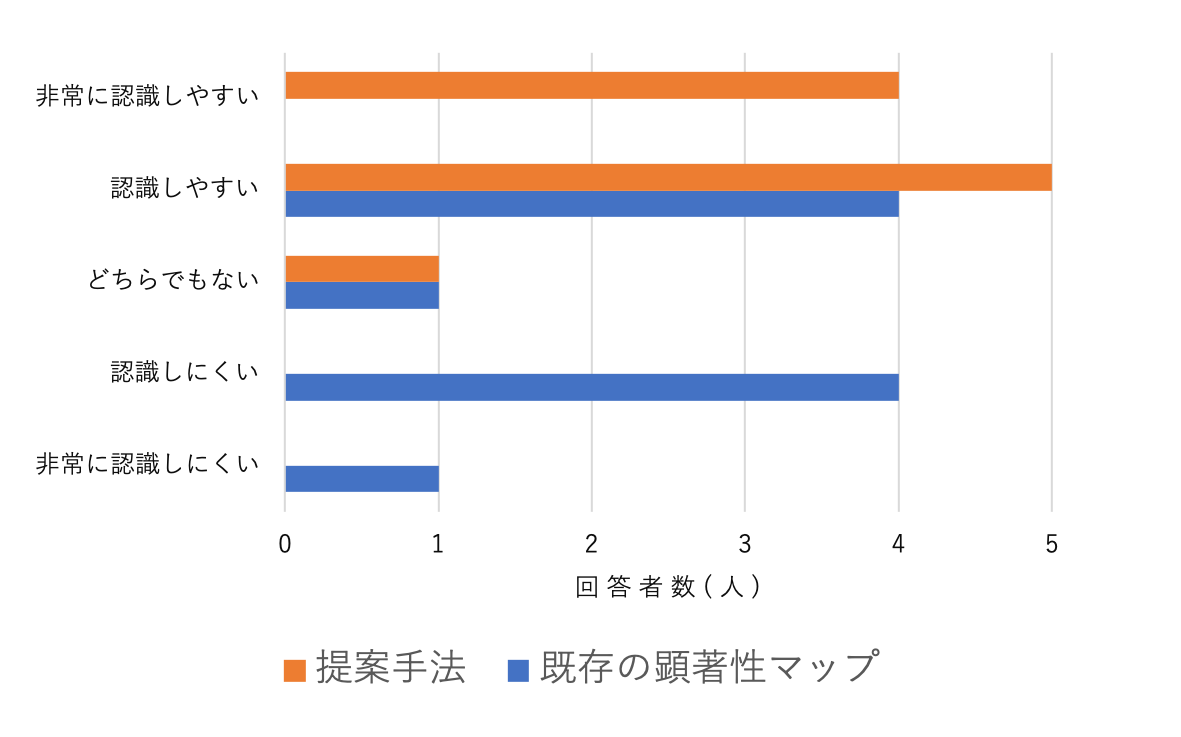
\includegraphics[width=10cm]{figures/result01.png}
    \caption{重要領域の認識のしやすさに関する評価結果}
    \label{fig_evaluation02-1}
\end{figure}

\subsubsection{集約図の効果に関する評価}
\par 3つ目の評価方法では特に顕著度が高い重要領域をタイル状に並べてまとめた集約図の効果について評価した。図\ref{fig_experience03-1}に示す集約図を見てウェブページの内容を予想してもらう問いでは、「食品系を取り扱う企業のホームページ」というざっくりしたページの内容は被験者全員が分かるものの、「関東に展開するスーパーを展開する企業」などのより詳細な内容は理解するのは難しいように感じた。
\par 次に、表\ref{table:evaluation03-1}にQ8の重要領域のみを抽出した集約図を見てどの程度ウェブページの内容を判断できるかを質問した結果を、表\ref{table:evaluation03-2}にQ9の初見のウェブページの内容を一目で確認したい時に集約図は効果的だと思うかを質問した結果を示す。Q8の結果を見ると「少し判断できる」と「ある程度判断できる」に意見が集まり、「ほとんど判断できる」は回答者がいなかった。また、Q9の結果を見ると「あまり効果的でない」が2名、「どちらでもない」が2名、「効果的である」が6名で「非常に効果的である」は回答者がいなかった。以上の結果から提案した集約図を見る事でページ内容をある程度は判断できるものの非常に効果があるとは言えないことが明らかになり、ウェブページの内容理解支援ツールとしては改善が必要であると言える。

\begin{table}[H]
    \caption{Q8の回答結果}
    \label{table:evaluation03-1}
    \centering
     \begin{tabular}{lc}
      \hline
      選択肢 & 回答数 \\
      \hline \hline
      全く判断できない & 0 \\
      少し判断できる & 2 \\
      ある程度判断できる & 8 \\
      ほとんど判断できる & 0 \\
      \hline
    \end{tabular}
\end{table}

\begin{table}[H]
    \caption{Q9の回答結果}
    \label{table:evaluation03-2}
    \centering
     \begin{tabular}{lc}
      \hline
      選択肢 & 回答数 \\
      \hline \hline
      全く効果的でない & 0 \\
      あまり効果的でない & 2 \\
      どちらでもない & 2 \\
      効果的である & 6 \\
      非常に効果的である & 0 \\
      \hline
    \end{tabular}
\end{table}